\documentclass[]{beamer}
\usepackage[T1]{fontenc}
\usepackage[utf8]{inputenc}
\usepackage{lmodern}
\usepackage[italian]{babel}

\title{Database}
\author{Mattia Cozzi\newline\href{mailto:cozzimattia@gmail.com}{\texttt{cozzimattia@gmail.com}}}
\date{a.s.~2023/2024}


%\documentclass[handout]{beamer}     %usare questa classe per generare l'handout

%\usepackage{pdfpages}   %per mostrare più quadri nella stessa pagina
%\pgfpagesuselayout{4 on 1}[a4paper,border shrink=5mm,landscape]


\usetheme{Singapore}
%\useoutertheme[left]{sidebar} %elementi intorno alle diapositive
\setbeamercovered{dynamic} %modifica l'aspetto del testo grigetto delle diapositive future. Argomenti: invisible/transparent/dynamic


%COLORE PRINCIPALE
\definecolor{verde}{RGB}{2, 194, 117} % UBC Blue (primary)
\setbeamercolor{structure}{fg=verde} % itemize, enumerate, etc
\setbeamercolor{alerted text}{fg=verde}


\usecolortheme{orchid}

\usepackage{tikz}

\begin{document}

\begin{frame}
  \titlepage
\end{frame}


\begin{frame}
\frametitle{Contenuti}
\tableofcontents
\end{frame}



\section{Introduzione}


\begin{frame}
\frametitle{Basi di dati}
Nelle applicazioni informatiche sono presenti informazioni che è necessario memorizzare in modo permanente per renderle utilizzabili per elaborazioni. Inoltre, quando molti utenti lavorano su un insieme di dati, è necessario avere una sola copia dei dati, sempre aggiornata, che consenta l'accesso simultaneo a più utenti. Questo compito è svolto dai \alert<1>{database} (basi di dati). 

~

Le \alert<2>{basi di dati} sono raccolte di dati progettati in modo tale da poter essere utilizzati in maniera ottimizzata da diverse applicazioni e diversi utenti.\pause

~

Il sistema che gestisce i dati e la loro organizzazione è detto \alert<3>{DBMS} (DataBase Management System).
\end{frame}


\begin{frame}
\frametitle{Funzioni di un DBMS}
Un DBMS deve:
\begin{itemize}
  \item gestire grandi quantità di dati, senza essere un ``collo di bottiglia'';\pause
  \item garantire la condivisione dei dati, ad esempio coordinando gli accessi;\pause
  \item garantire la persistenza dei dati e la loro integrità, controllando gli accessi;\pause
  \item avere un'interfaccia grafica per l'amministrazione dei dati.
\end{itemize}
\end{frame}


\begin{frame}
\frametitle{Esempi di DBMS}
Commerciali:
\begin{itemize}
  \item Oracle;
  \item MS SQL Server;
  \item MS Access (inserito nel pacchetto MS Office).
\end{itemize}\pause

~

Open source:
\begin{itemize}
  \item MySQL;
  \item PostgreSQL;
  \item Base (inserito nel pacchetto LibreOffice).
\end{itemize}
\end{frame}

\begin{frame}
\frametitle{Schema riassuntivo}
\begin{figure}
  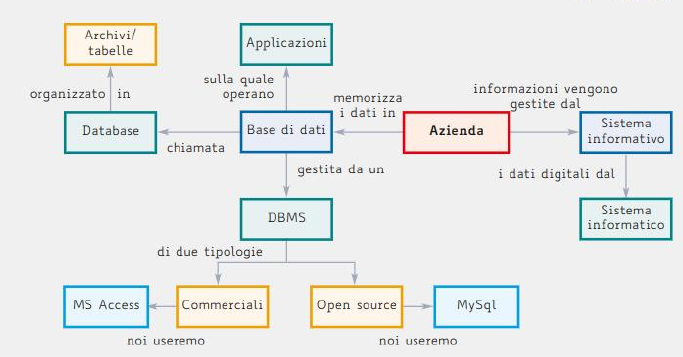
\includegraphics[width=\columnwidth]{img/schemadb.png}
\end{figure}
\end{frame}


\begin{frame}
\frametitle{Fasi della progettazione di un database}
La creazione di un database è un'operazione complessa, che viene svolta con una metodologia precisa:

~

\begin{enumerate}
  \item modellazione dei dati (creazione delle tabelle):\pause
  \begin{enumerate}
    \item analisi;\pause
    \item progettazione concettuale mediante il modello E-R (COSA);\pause
    \item progettazione logica mediante lo schema logico o modello relazionale (COME);\pause
  \end{enumerate}

  ~

  \item modellazione funzionale:
  \begin{enumerate}
    \item implementazione;
    \item realizzazione delle applicazioni.
  \end{enumerate}
\end{enumerate}
\end{frame}




\begin{frame}
\frametitle{Modello relazionale}
Il modello maggiormente utilizzato per rappresentare i dati è il \alert<1>{modello relazionale}, che si realizza mediante tabelle.\pause

~

Le colonne delle tabelle rappresentano campi o proprietà, le righe rappresentano i diversi record.

\begin{figure}
  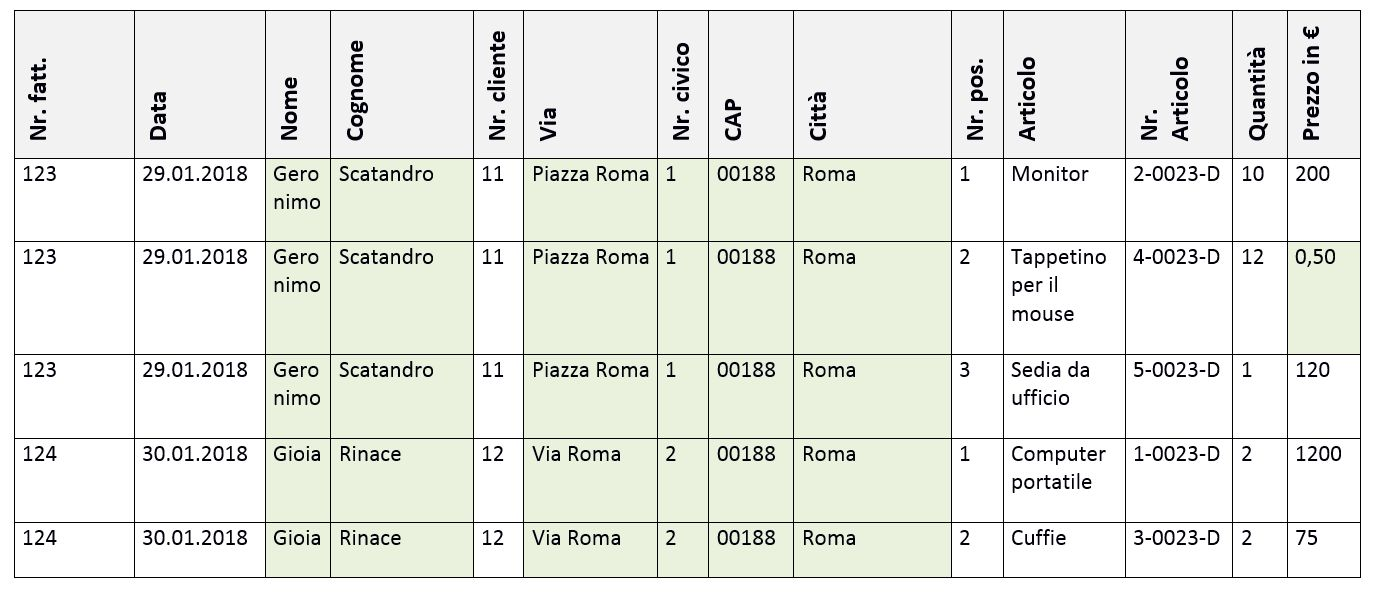
\includegraphics[width=.9\columnwidth]{img/tabelladb.jpg}
\end{figure}
\end{frame}

\section{Entità}

\begin{frame}
\frametitle{Modello Entità-Relazione}
Questo modello permette di modella graficamente il mondo reale sotto forma di \alert<1>{entità} e \alert<1>{relazioni} tra esse.\pause

~

Le entità sono gli oggetti principali su cui vengono raccolte le informazioni. Ogni entità rappresenta graficamente un oggetto, concreto o astratto, del mondo reale.\pause

~

Ogni entità avrà un nome, che permette di identificare ogni \alert<3>{istanza} (ogni ``esemplare'') di quella classe.\pause

~

Le relazioni tra entità verranno rappresentate mediante linee che collegano le entità.
\end{frame}


\begin{frame}
\frametitle{Rappresentazione delle entità}
Le entità possono essere rappresentate in \alert<1>{notazione classica}:
\begin{figure}
  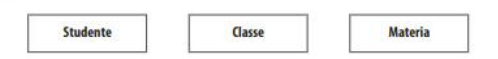
\includegraphics[width=.6\columnwidth]{img/entitastd.png}
\end{figure}
oppure in \alert<1>{notazione UML} (Unified Modelling Language):
\begin{figure}
  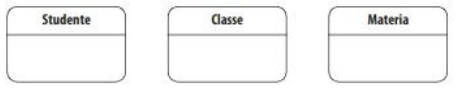
\includegraphics[width=.6\columnwidth]{img/entitauml.png}
\end{figure}
\end{frame}



\begin{frame}
\frametitle{Tipi di entità}
Possiamo distinguere tra \alert<1>{entità forti} (che non richiedono altre entità per essere identificata) e \alert<1>{entità deboli}.\pause

~

Ad esempio, in un database ospedaliero, ``Paziente'' è entità forte, ``Esame'' è entità debole.\pause

~

Esistono inoltre \alert<3>{entità associative}, usate per associare due o più entità tra loro, cioè per risolvere delle associazioni multiple.\pause

~

Ad esempio, in un database di classe, ogni ``Docente'' insegna in diverse ``Classi'', e serve pertanto l'entità ``Orario'' per associare ogni docente alle sue classi.
\end{frame}



\begin{frame}
\frametitle{Istanze}
Ogni istanza di una certa entità è caratterizzato da un \alert<1>{insieme di valori che descrivono le sue proprietà}.\pause

~

Tutte le istanze di una certa entità hanno gli stessi attributi, ma con valori diversi per poterle distinguere.\pause

~

Ad esempio, er l'entità ``Studente'', gli attributi possono essere ``Nome'', ``Cognome'', ``Codice fiscale'', ``Data di nascita'', ``Sezione'', ecc.
\end{frame}


\section{Attributi}

\begin{frame}
\frametitle{Attributi}
Attributo fondamentale di ogni istanza è il suo identificatore univoco, detto \alert<1>{chiave}.\pause

~

I tipi di attributi sono mostrati in figura.
\begin{figure}
  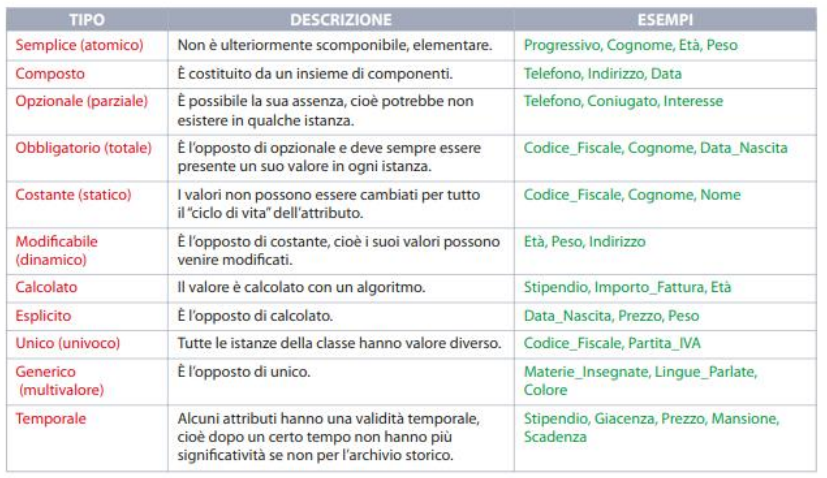
\includegraphics[width=.9\columnwidth]{img/tabellaattributi.png}
\end{figure}
\end{frame}


\begin{frame}
\frametitle{Dominio degli attributi}
In fase di progettazione è importante stabilire quali specifiche devono rispettare gli attributi:
\begin{itemize}
  \item tipo di dato: intero, decimale, carattere (stringa di caratteri), più i tipi speciali per data, ora e valori logici (booleani);\pause
  \item lunghezza e obbligatorietà;\pause
  \item se il valore NULL è supportato e se esiste un valore di default;\pause
  \item intervallo: indica i limiti inferiori e superiori dei valori.
\end{itemize}\pause

~

Sugli attributi possono anche essere impostati specifici \alert<5>{vincoli}, particolari restrizioni o controlli sui valori ammessi.

~

Il controllo della correttezza degli attributi è detto \alert<6>{validazione}.
\end{frame}



\begin{frame}
\frametitle{Esempio di definizione degli attributi}
Per l'entità ``Persona'':
\begin{itemize}
  \item Nome: stringa(20), obbligatorio, non NULL
  \item Cognome: stringa(20), obbligatorio, non NULL
  \item Cod\_Fiscale: stringa(16)
  \item Titolo\_di\_Studio: stringa(50)
  \item Data\_di\_Nascita: giorno - mese - anno
  \item Peso: numerico
  \item Anzianità\_Servizio: numerico
\end{itemize}
\end{frame}

\begin{frame}
\frametitle{Rappresentazione degli attributi}
Gli attributi possono essere rappresentati in \alert<1>{notazione classica}:
\begin{figure}
  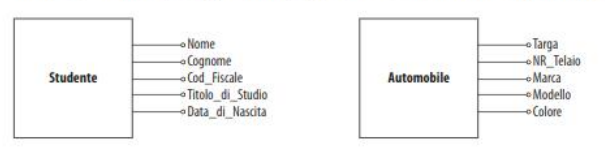
\includegraphics[width=.8\columnwidth]{img/attributistd.png}
\end{figure}
oppure in \alert<1>{notazione UML}:
\begin{figure}
  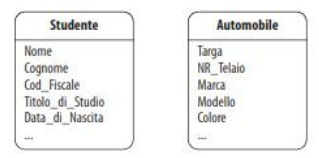
\includegraphics[width=.5\columnwidth]{img/attributiuml.png}
\end{figure}
\end{frame}


\begin{frame}
\frametitle{Schema riassuntivo}
\begin{figure}
  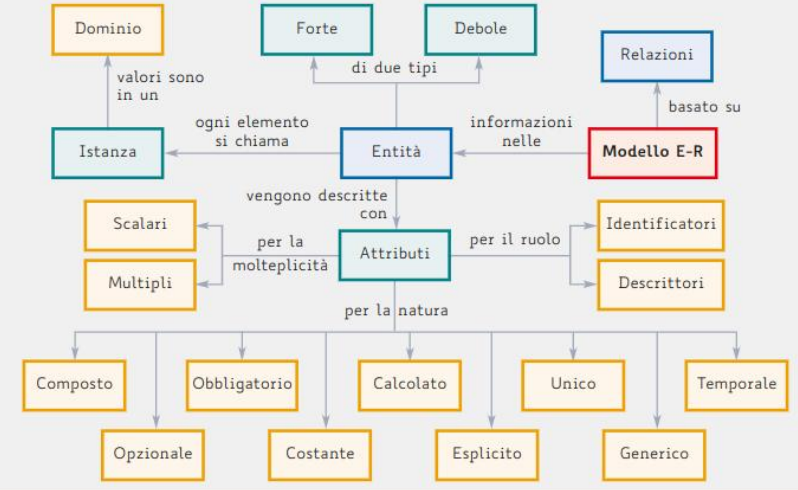
\includegraphics[width=\columnwidth]{img/schemaattributi.png}
\end{figure}
\end{frame}


\section{Chiavi}


\begin{frame}
\frametitle{Attributi chiave}
Gli attributi chiave sono degli \alert<1>{identificatori univoci} di un'istanza di un'entità. Ogni attributo chiave (\emph{primary key}):
\begin{itemize}
  \item deve essere obbligatorio, unico, esplicito (vedi tabella precedente);\pause
  \item può essere semplice o composto;\pause
  \item non deve essere modificabile;\pause
  \item non può avere valore NULL.\pause
\end{itemize}

~

Rappresentazione degli attributi chiave:
\begin{columns}
\begin{column}{.4\textwidth}
  \begin{figure}
    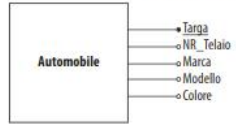
\includegraphics[width=.8\columnwidth]{img/chiavestd.png}
  \end{figure}
\end{column}
\begin{column}{.4\textwidth}
  \begin{figure}
    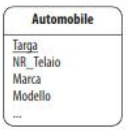
\includegraphics[width=.5\columnwidth]{img/chiaveuml.png}
  \end{figure}
\end{column}
\end{columns}
\end{frame}


\begin{frame}
\frametitle{Chiavi artificiali}
Una chiave artificiale è un attributo che assegna un \alert<1>{codice univoco} ad ogni istanza.\pause

~

Esempio: la numerazione sequenziale delle tessere rilasciate da una associazione.\pause

~

La maggior parte dei DBMS ammette il tipo contatore: gli attributi definiti come contatore si \alert<3>{autoincrementano di 1 per ogni record che viene aggiunto}.\pause

~

Alle chiavi artificiali viene solitamente dato un nome che inizia con \alert<4>{ID\_} (ID\_Studente, ID\_Auto).
\end{frame}


\begin{frame}
\frametitle{Chiavi esterne}
Le chiavi esterne (\emph{foreign keys}) sono utilizzate per \alert<1>{realizzare i collegamenti} tra entità, risolvendo quindi i collegamenti uno-a-molti.\pause

~

Se le chiavi esterne sono chiavi artificiali, vengono nominate in modo simile a quanto si fa per le chiavi primarie, con il prefisso \alert<2>{id\_} (minuscolo).\pause

~

\visible<3->{
\begin{figure}
  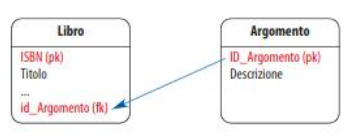
\includegraphics[width=.6\columnwidth]{img/chiaviesterneuml.png}
\end{figure}
}
\end{frame}


\section{Relazioni}

\begin{frame}
\frametitle{Relazioni}
Ogni associazione \alert<1>{binaria} ha:
\begin{itemize}
  \item un'entità di partenza e una di arrivo;\pause
  \item una descrizione che ne esprima il significato;\pause
  \item eventuali attributi caratterizzanti.\pause
\end{itemize}

~

Rappresentazione delle relazioni:
\visible<4>{\begin{figure}
  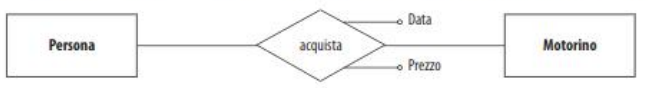
\includegraphics[width=.8\columnwidth]{img/relazionestd.png}

  ~

  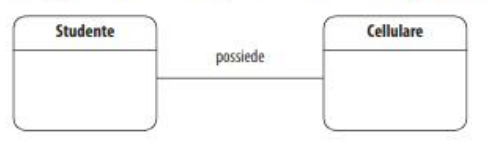
\includegraphics[width=.5\columnwidth]{img/relazioneuml.png}
\end{figure}}
\end{frame}


\begin{frame}
\frametitle{Cardinalità delle relazioni}
Una relazione può essere:
\begin{itemize}
  \item \alert<1>{uno-a-uno (1,1)}, espressa da una funzione biettiva tra due insiemi che contengono le istanze da associare;\pause
  \visible<1->{\begin{figure}
    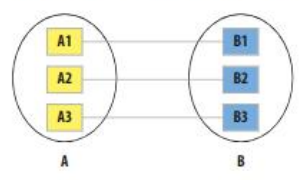
\includegraphics[width=.3\columnwidth]{img/card11.png}
  \end{figure}}
  \item \alert<2>{uno-a-molti (1, n)};
  \visible<2->{\begin{figure}
    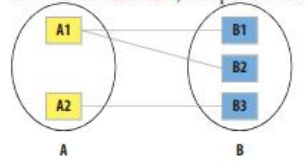
\includegraphics[width=.3\columnwidth]{img/card1n.png}
  \end{figure}}\pause
  \item \alert<3>{molti-a-molti (n, n)}.
\end{itemize}
\end{frame}

\begin{frame}
\frametitle{Rappresentazione della cardinalità delle relazioni (classica)}
\begin{figure}
  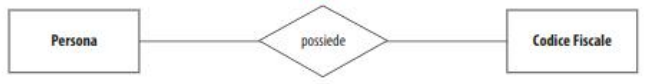
\includegraphics[width=.9\columnwidth]{img/card11std.png}

  ~

  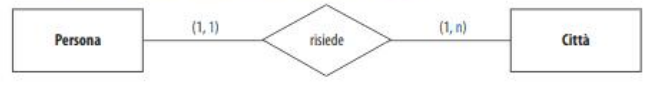
\includegraphics[width=.9\columnwidth]{img/card1nstd.png}

  ~

  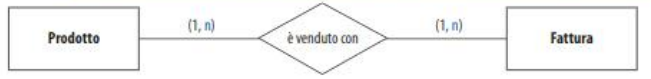
\includegraphics[width=.9\columnwidth]{img/cardnnstd.png}
\end{figure}
\end{frame}


\begin{frame}
\frametitle{Rappresentazione della cardinalità delle relazioni (UML)}
\begin{figure}
  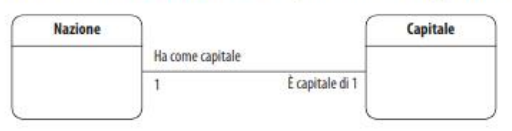
\includegraphics[width=.7\columnwidth]{img/card11uml.png}

  ~

  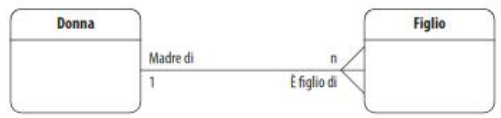
\includegraphics[width=.7\columnwidth]{img/card1numl.png}

  ~

  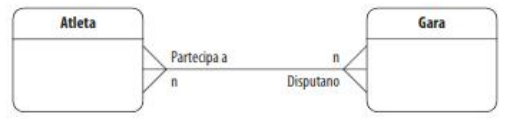
\includegraphics[width=.7\columnwidth]{img/cardnnuml.png}
\end{figure}
\end{frame}


\begin{frame}
\frametitle{Esempio di diagramma E-R}
\begin{figure}
  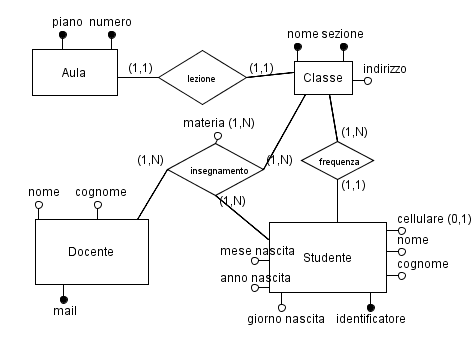
\includegraphics[width=.8\columnwidth]{img/esempioer.png}
\end{figure}
\end{frame}

\section{Progettazione}

\begin{frame}
\frametitle{Realizzazione di un database}
La progettazione è solitamente svolta da un \alert<1>{database designer}, responsabile dell'astrazione dei dati dal mondo reale a partire dall'analisi dei requisiti fino alla corretta modellazione.\pause

~

Il primo passo è la realizzazione dello \alert<2>{schema concettuale}, ovvero del \alert<2>{diagramma E-R}, inizialmente in forma provvisoria, poi via via più raffinata.\pause

~

È necessario:
\begin{itemize}
  \item \alert<3>{definire gli oggetti} del diagramma, eventualmente realizzando un glossario;\pause
  \item completare le entità con i loro \alert<4>{attributi};\pause
  \item individuare le \alert<5>{relazioni} esistenti tra le entità.
\end{itemize}
\end{frame}



\begin{frame}
\frametitle{Schema di progettazione di un database}
\begin{figure}
  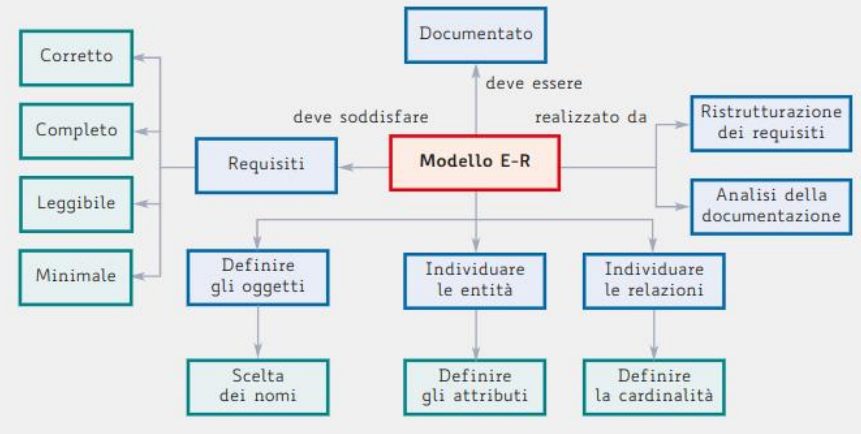
\includegraphics[width=\columnwidth]{img/schemaprogettodb.png}

  ~

  \href{https://drive.google.com/file/d/1CgjeBq9g0px8xHsf9-F2KneF8EB-yGiY/view?usp=share_link}{\beamergotobutton{Esempio di progettazione di un database}}
\end{figure}
\end{frame}

\begin{frame}
\frametitle{Realizzazione dello schema logico}
Il modello (o schema) logico viene utilizzato come input per la progettazione vera e propria del database: deve avere quindi il massimo livello di dettaglio e precisione possibile.\pause

~

Deve contenere tutte le informazioni necessarie per definire le tabelle, riportando la descrizione puntuale e completa del significato di ogni dato memorizzato.\pause

~

\alert<3>{Lo schema logico trasforma le informazioni del modello concettuale in un formato efficiente.}\pause

~

Utilizzeremo un modello relazionale,e dovremo quindi definire le \alert<4>{tabelle relazionali}.
\end{frame}


\begin{frame}
\frametitle{Mappatura}
La traduzione delle tabelle dallo schema concettuale allo schema logico è un'operazione chiamata \emph{mapping} (mappatura).

~

Un modello logico preciso comprende:
\begin{itemize}
  \item per ogni entità:
  \begin{itemize}
    \item l'elenco completo degli attributi;
    \item l'indicazione della chiave primaria;
    \item l'indicazione di eventuali chiavi esterne;
  \end{itemize}
  \item per ogni attributo:
  \begin{itemize}
    \item l'indicazione di opzionalità o di obbligatorietà;
    \item l'indicazione del tipo di dati e dei valori ammessi;
  \end{itemize}
  \item per ogni relazione:
  \begin{itemize}
    \item l'indicazione della molteplicità minima e massima in entrambe le direzioni;
    \item l'indicazione delle regole di integrità referenziale applicabili.
  \end{itemize}
\end{itemize}
\end{frame}


\begin{frame}
\frametitle{Dallo schema concettuale allo schema logico}
Il passaggio dallo schema E-R allo schema logico comprende due fasi:
\begin{enumerate}
  \item ristrutturazione del diagramma E-R;\pause
  \item traduzione del modello E-R nello schema logico e nelle tabelle relazionali.
\end{enumerate}

~

\visible<3->{\begin{figure}
  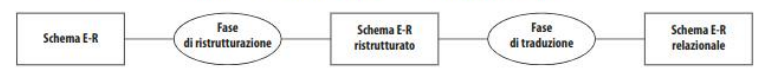
\includegraphics[width=\columnwidth]{img/ristrutturazione.png}
\end{figure}}
\end{frame}



\begin{frame}
\frametitle{Ristrutturazione}
La ristrutturazione avviene secondo le seguenti regole:
\begin{enumerate}
  \item \alert<1->{Partecipazione delle entità alle relazioni:} ogni entità creata deve essere collegata a qualche altra entità, altrimenti non sarà possibile collegare quella tabella alle altre. \pause
  \item \alert<2->{Eliminazione degli attributi composti e aggiunta di attributi semplici}: se sono presenti attributi composti, essi vanno eliminati e sostituiti con attributi semplici.\pause
  \item \alert<3>{Eliminazione degli attributi multivalore e aggiunta di entità}: gli eventuali attributi multivalore devono essere ``promossi'' a entità, creando cioè una nuova entità che contenga i valori dell'attributo e collegandola all'entità che possedeva l'attributo mediante una nuova relazione opportuna.
\end{enumerate}
\end{frame}


\begin{frame}
\frametitle{Esempio: attributo multivalore}
Ad esempio, prima della ristrutturazione:
\begin{figure}
  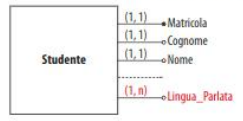
\includegraphics[width=.35\columnwidth]{img/ristrutturazione1.png}
\end{figure}\pause
Dopo la ristrutturazione:
\visible<2>{
  \begin{figure}
    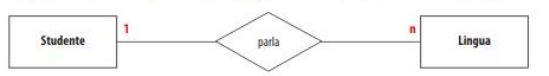
\includegraphics[width=.9\columnwidth]{img/ristrutturazione2.png}
  \end{figure}
}
\end{frame}



\begin{frame}
\frametitle{Semplificazione (1)}
Dopo aver ottenuto lo schema ristrutturato, possiamo tradurlo nel modello/schema relazionale.

~

Si seguono le seguenti regole:
\begin{enumerate}
  \item \alert<1>{Trasformazione delle entità}: per ogni entità viene generata una tabella indicando lo schema relazionale, in cui viene riportato un campo per ogni attributo dell'entità.
  
  Il diagramma E-R:
  \begin{figure}
    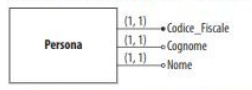
\includegraphics[width=.4\columnwidth]{img/ristrutturazione3.png}
  \end{figure}
  viene tradotto nel seguente schema relazionale:
    \begin{figure}
      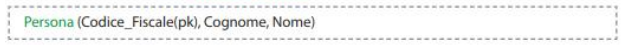
\includegraphics[width=.9\columnwidth]{img/ristrutturazione4.png}
    \end{figure}
\end{enumerate} 
\end{frame}


\begin{frame}
\frametitle{Semplificazione (2)}
\begin{enumerate}\setcounter{enumi}{1}
  \item \alert<1>{Trasformazione delle relazioni}: si procede in base al numero di entità partecipanti e alla loro cardinalità.\pause
  
  ~

  \begin{itemize}
    \item \alert<2>{Unificare le relazioni uno-a-uno}: se due entità sono collegate da una relazione (1,1), possono essere ridotte ad un'unica entità che contiene gli attributi sia della prima sia della seconda entità.\pause
    
    ~

    \item \alert<3>{Eliminare le relazioni complesse}, che coinvolgono più di una entità, riducendole a relazioni binarie.\pause
    
    ~

    \item \alert<4>{Semplificare le relazioni molti-a-molti}: le relazioni molti-a-molti non sono supportate nel modello relazionale e devono essere sostituite creando un'entità associativa che va messa in relazione con le due entità originali.
  \end{itemize}
\end{enumerate} 
\end{frame}


\begin{frame}
\frametitle{Semplificazione (3)}
Ad esempio, prima della semplificazione:
\begin{figure}
  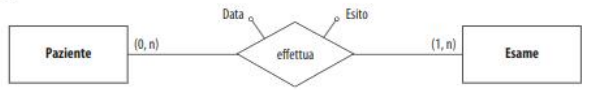
\includegraphics[width=.7\columnwidth]{img/ristrutturazione5.png}
\end{figure}
Dopo la semplificazione:
\begin{figure}
  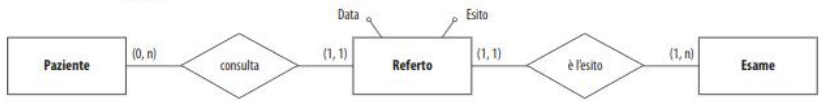
\includegraphics[width=\columnwidth]{img/ristrutturazione6.png}
\end{figure}
Nello schema relazionale otteniamo:
\begin{figure}
  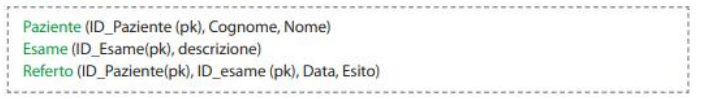
\includegraphics[width=.9\columnwidth]{img/ristrutturazione7.png}

  ~

  \href{https://drive.google.com/file/d/1JC_u1LHESKUEAs66X9ybOHXqbAzYluJ5/view?usp=share_link}{\beamergotobutton{Progettazione schema logico di un database}}
\end{figure}
\end{frame}


\begin{frame}
\frametitle{Schema riassuntivo}
\begin{figure}
  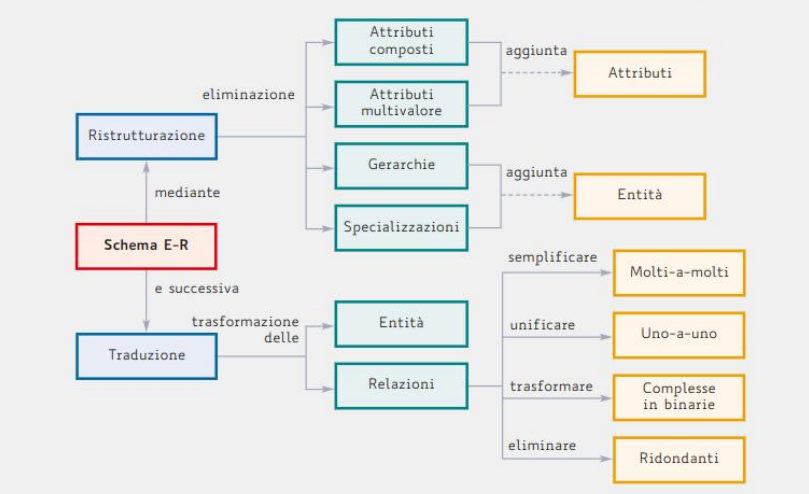
\includegraphics[width=\columnwidth]{img/schemaprogettazionedb.png}
\end{figure}
\end{frame}


\section{Traduzione}


\begin{frame}
\frametitle{Tabelle relazionali (1)}
Il modello relazionale, introdotto da E.F.~Codd nel 1970, presenta i dati nella forma di \alert<1>{tabelle bidimensionali}.\pause

~

Ogni tabella ha:
\begin{itemize}
  \item un nome per ogni colonna;\pause
  \item un elenco di colonne di cui vengono specificati i tipi;\pause
  \item una \alert<4>{chiave primaria} che identifica univocamente ogni riga della tabella.\pause
\end{itemize}

~

Tra due o più colonne di tabelle ci può essere una relazione: le due tabelle sono allora collegate tramite \alert<5>{chiavi esterne}.
\end{frame}


\begin{frame}
\frametitle{Terminologia}
Le colonne possono anche essere chiamate ``campi'' o ``attributi'', mentre le righe possono anche essere chiamate ``record'' o ``tuple''.

~

\begin{figure}
  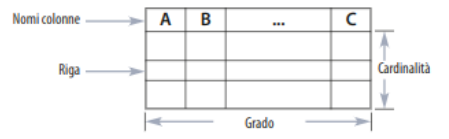
\includegraphics[width=.75\columnwidth]{img/tabellaterminologia.png}
\end{figure}
\end{frame}


\begin{frame}
\frametitle{Traduzione (1)}
Seguiamo queste quattro regole:
\begin{enumerate}
  \item ogni entità diventa una tabella;\pause
  \item ogni attributo dell'entità diventa una colonna della tabella;\pause
  \item ogni istanza di un'entità diventa una riga della tabella;\pause
  \item la chiave primaria dell'entità è l'identificatore univoco delle righe di una tabella;\pause
  \item le relazioni sono rappresentate con chiavi esterne che collegano righe di due diverse tabelle.\pause
\end{enumerate}
\end{frame}


\begin{frame}
\frametitle{Traduzione (2)}
Ad esempio, se nello schema concettuale abbiamo:
\begin{figure}
  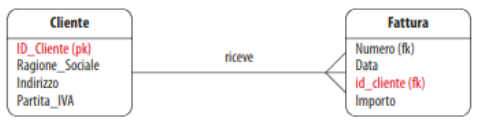
\includegraphics[width=.7\columnwidth]{img/ristrutturazione8.png}
\end{figure}
nello schema logico otteniamo:
\begin{figure}
  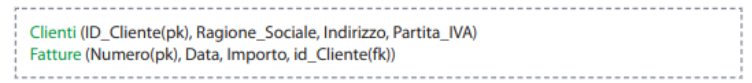
\includegraphics[width=.9\columnwidth]{img/ristrutturazione9.png}
\end{figure}
\end{frame}

\begin{frame}
\frametitle{Traduzione (3)}
Si è soliti, passando allo schema logico, inserire la chiave primaria nella prima colonna a sinistra, mentre le chiavi esterne nelle ultime colonne a destra.
\begin{figure}
  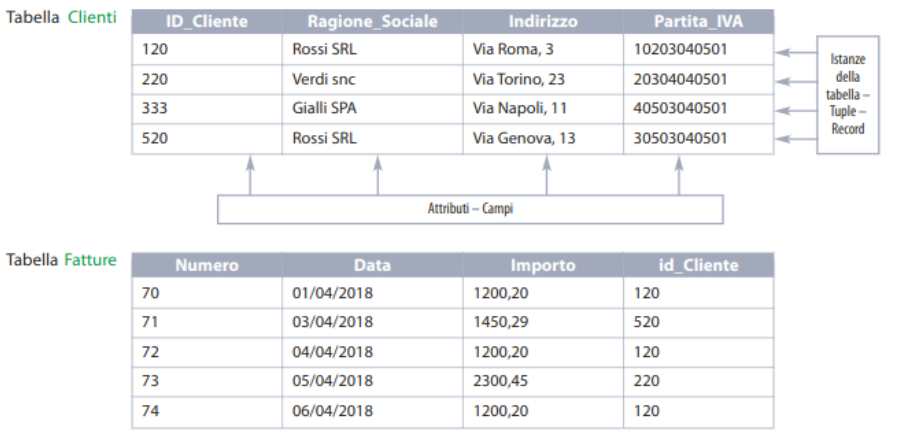
\includegraphics[width=.95\columnwidth]{img/ristrutturazione10.png}
\end{figure}
\end{frame}


\begin{frame}
\frametitle{Tabelle relazionali (2)}
Le tabelle relazionali hanno le seguenti proprietà:
\begin{itemize}
  \item i valori sono atomici, non ulteriormente scomponibili;\pause
  \item i valori di una colonna sono \alert<2>{dello stesso tipo};\pause
  \item \alert<3>{ogni riga è univoca}, diversa dalle altre (garantito dalla presenza di una chiave primaria);\pause
  \item l'ordine di righe o colonne non è rilevante (permette di aggiungere righe o colonne successivamente alla creazione del database);\pause
  \item ogni colonna ha un nome univoco.\pause
\end{itemize}
\end{frame}


\begin{frame}
\frametitle{Esempio}
Per un database bibliografico con il seguente schema concettuale:
\begin{figure}
  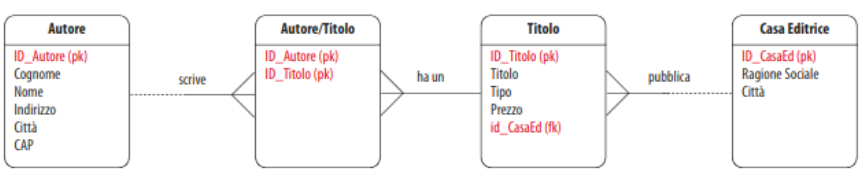
\includegraphics[width=\columnwidth]{img/ristrutturazione11.png}
\end{figure}
si ottiene il seguente schema relazionale:
\begin{figure}
  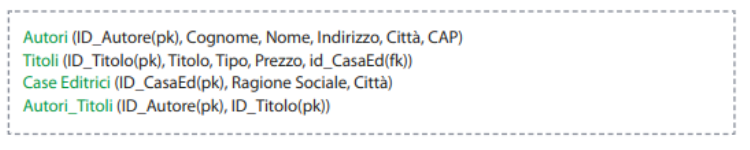
\includegraphics[width=.9\columnwidth]{img/ristrutturazione12.png}
\end{figure}
\end{frame}



\begin{frame}
\frametitle{Riempire (popolare) le tabelle}
\begin{figure}
  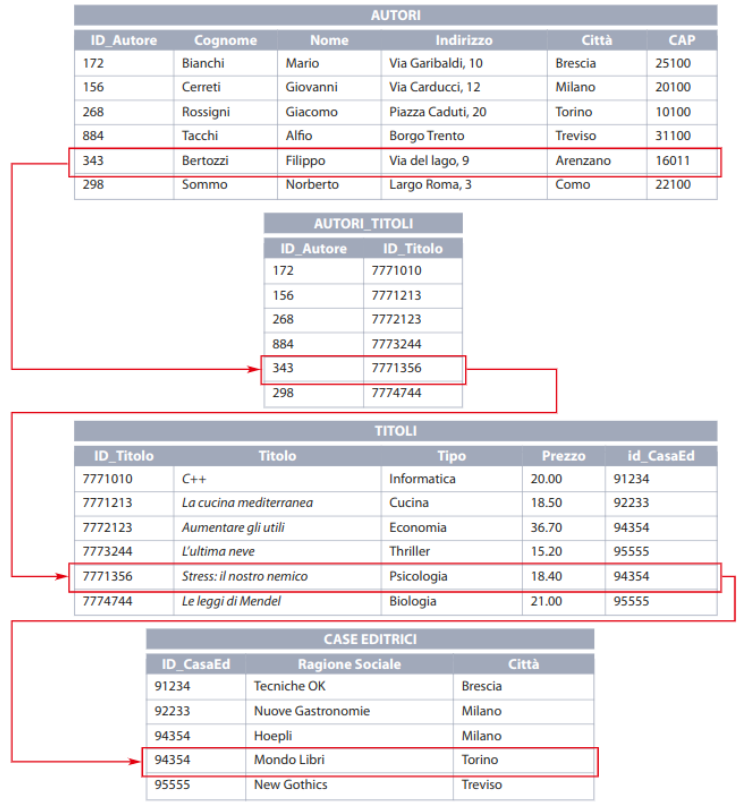
\includegraphics[width=.6\columnwidth]{img/ristrutturazione13.png}
\end{figure}
\end{frame}



\begin{frame}
\frametitle{Schema riassuntivo}
\begin{figure}
  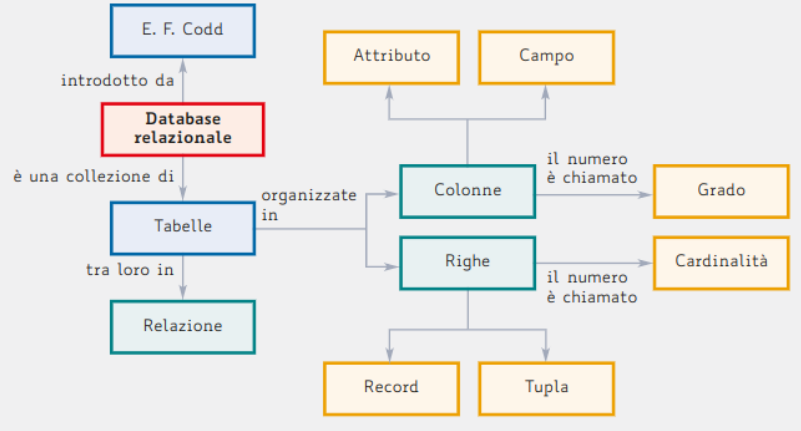
\includegraphics[width=\columnwidth]{img/schemadb1.png}
\end{figure}
\end{frame}


\begin{frame}
\frametitle{Regole di integrità e normalizzazione}
\begin{center}
  \href{https://drive.google.com/file/d/1ZnmILMv5fum42uVRmkTTZmq5LovXvvpv/view?usp=share_link}{\beamergotobutton{Materiale completo sui database}}
\end{center}

~

Quando vengono eseguite operazioni sui dati presenti nel database, come inserimento, modifica o cancellazione, è necessario che vengano rispettate le definizioni del database. A tale scopo vengono fissate delle specifiche \alert<1>{regole di integrità} (cap.~9).\pause

~

La \alert<2>{normalizzazione} è un processo che tende a eliminare la ripetizione (ridondanza) dei dati e a migliorarne la consistenza. Questo processo punta a ottenere la tabella in ``forma normale'' (cap.~10).
\end{frame}



% \section{Operazioni}


% \begin{frame}
% \frametitle{}
% \begin{center}
%   \href{https://drive.google.com/file/d/1JC_u1LHESKUEAs66X9ybOHXqbAzYluJ5/view?usp=share_link}{\beamergotobutton{Operazioni su un database di libri}}
% \end{center}
% \end{frame}

% \begin{frame}
% \frametitle{Schema riassuntivo}
% \begin{figure}
%   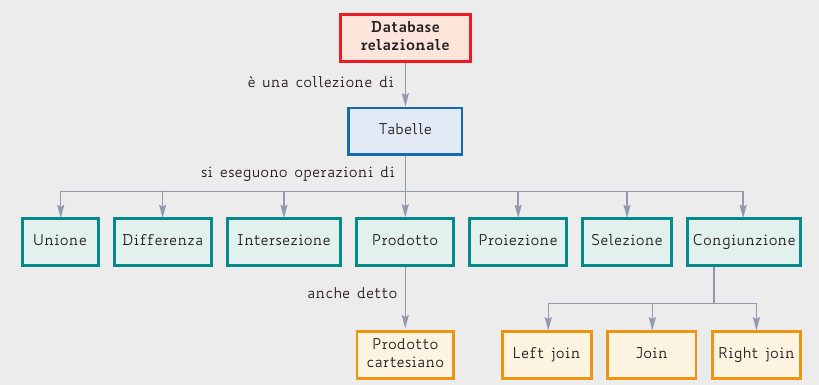
\includegraphics[width=\columnwidth]{img/schemaoperazioni.png}
% \end{figure}
% \end{frame}


\end{document}
